\documentclass{beamer}
\usetheme{metropolis}

\setbeamercolor{background canvas}{bg=white}

\usepackage[spanish]{babel}
\usepackage[utf8]{inputenc} % Codificación UTF-8
\usepackage{lmodern} % Fuente moderna para LaTeX
\usepackage{caption}

\title{Multi-modal recommender system for\\content streaming platforms}
\subtitle{Trabajo Final del Máster en Ciencia de Datos\\
Universitat Oberta de Catalunya}
\date{\today}
\author{José María Tagarro Martí}
\institute{Area: Data science in complex systems, sustainability and ecology\\Tutor: Francesc Julbe López\\Profesora: Susana Acedo Nadal}

\begin{document}

% Portada
\maketitle

% Índice
\begin{frame}{Índice}
    \tableofcontents
\end{frame}

% Introduction
\section{Introducción}
\begin{frame}{Contexto y motivación}
    \textbf{El mercado de \textit{streaming} enfrenta nuevos retos:}
    \begin{itemize}
        \item \textbf{Fragmentación del mercado:} El aumento de plataformas compitiendo por contenido exclusivo está reduciendo el control de cada plataforma sobre la calidad y amplitud de su catálogo.
        \item \textbf{Competencia creciente:} Las plataformas necesitan encontrar ventajas competitivas sostenibles que vayan más allá de su catálogo.
        \item \textbf{La experiencia del usuario como diferenciador:} 
        Mejorar las recomendaciones personalizadas es clave para retener usuarios y aumentar el engagement, creando una ventaja competitiva basada en factores que las plataformas sí pueden controlar.
    \end{itemize}
\end{frame}

% Problem Description
\section{Descripción del problema}

\begin{frame}{Descripción del problema}
    \begin{itemize}
        \item \textbf{Escalabilidad:} 
        Manejar recomendaciones personalizadas para catálogos con miles de títulos y millones de usuarios requiere algoritmos altamente eficientes y/o arquitecturas avanzadas.

        \item \textbf{Recomendaciones en tiempo real:} 
        Las sugerencias, como contenido relacionado tras ver una película, deben generarse en milisegundos para mejorar la experiencia del usuario.
        
        \item \textbf{\textit{Cold Start}:} 
        Es difícil recomendar contenido nuevo sin interacciones previas o a usuarios que apenas comienzan a usar la plataforma. Clave durante pruebas gratuitas promocionales.
        
        \item \textbf{\textit{Long Tail}:} 
        Gran parte del contenido del catálogo, menos popular pero potencialmente relevante, suele quedar fuera de las recomendaciones, afectando la diversidad y descubrimiento.
        
        
    \end{itemize}
\end{frame}

\begin{frame}{Problema de la larga cola}
    \begin{figure}
        \centering
        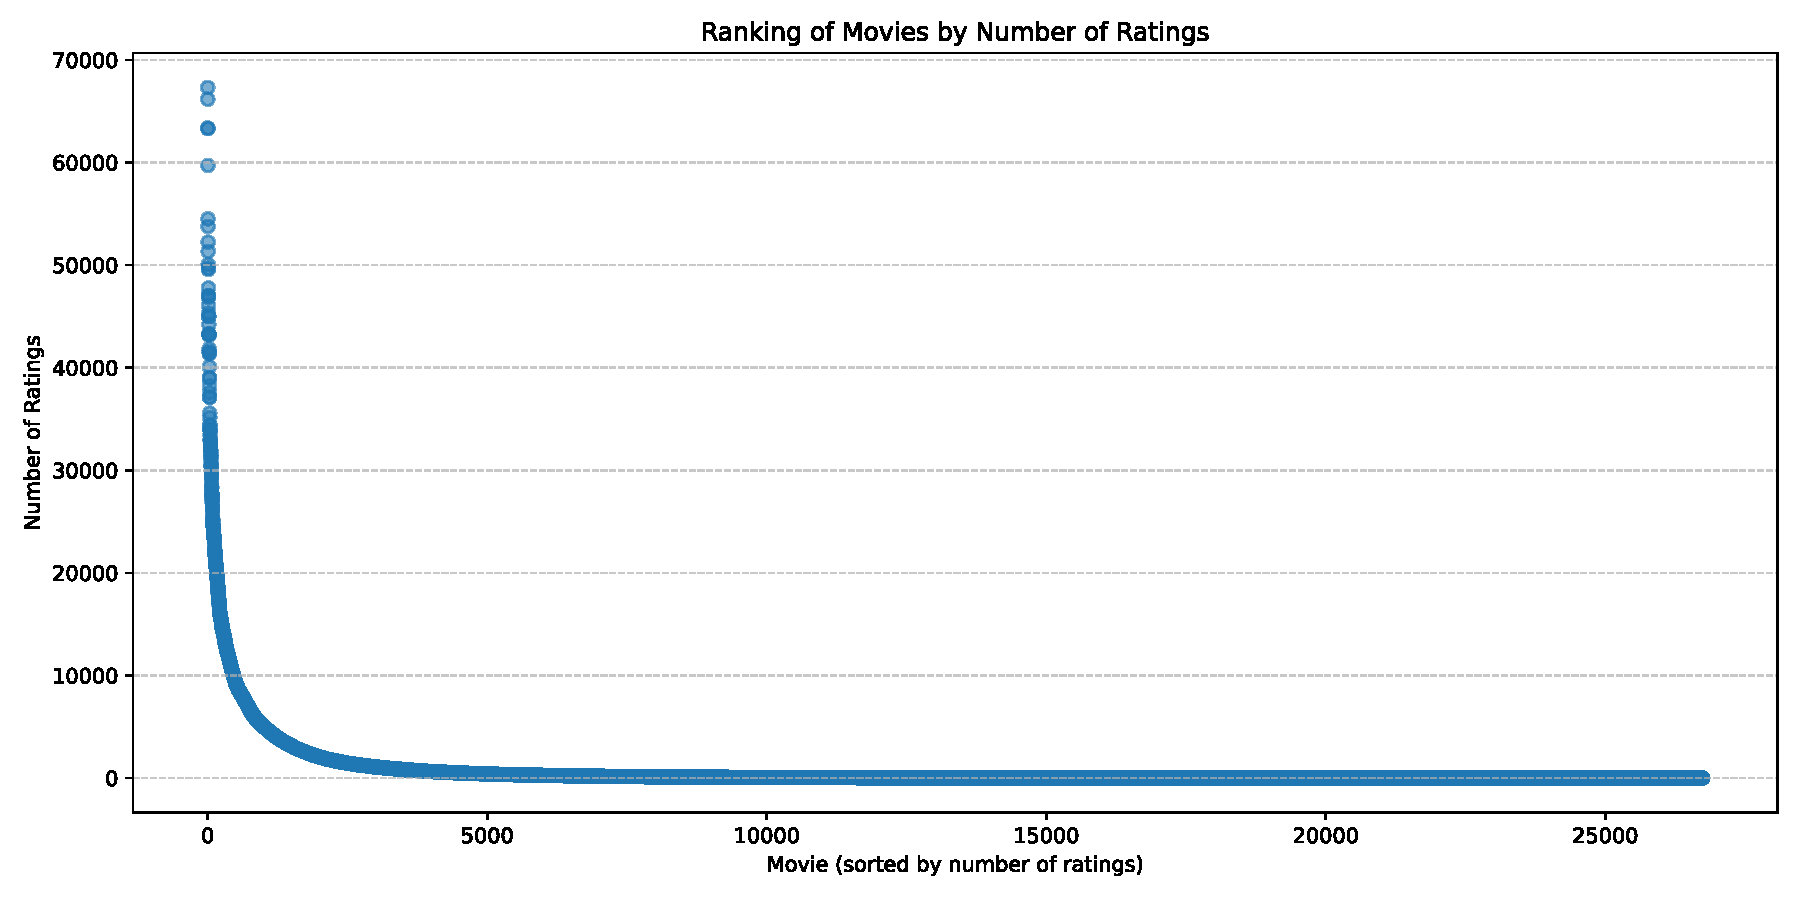
\includegraphics[width=\textwidth]{images/ranking_of_movies_by_ratings.pdf}
    \end{figure}
\end{frame}

% Goals and Contributions
\section{Objetivos y contribuciones}
\begin{frame}{Objetivos y contribuciones}
    \textbf{Objetivo principal:} Implementar un sistema de recomendación que otorgue una ventaja competitiva a las plataformas de contenidos. \\
    \vspace{0.5cm}
    \textbf{Contribuciones clave / innovaciones:}
    \begin{itemize}
        \item Primera aplicación de DMRL en plataformas de streaming.
        \item Creación de un dataset multimodal extendido basado en MovieLens-20M con inclusión de subtítulos y pósters.
        \item Exploración del impacto de las nuevas modalidades en los problemas de \textit{cold start} y \textit{long tail}.
    \end{itemize}
\end{frame}

% Dataset Description
\section{Descripción del dataset}

\begin{frame}{Métricas del dataset}
    \begin{itemize}
        \item \textbf{Número total de películas:} 27.278
        \item \textbf{Número total de usuarios:} 138.493
        \item \textbf{Número total de interacciones (ratings):} 20.000.263
        \item \textbf{Pósters disponibles:} 26.938 (99\%)
        \item \textbf{Subtítulos disponibles:} 22.473 (78\%)
    \end{itemize}
\end{frame}

\begin{frame}{Proceso de integración del dataset}
    \begin{figure}
        \centering
        \usetikzlibrary{positioning, arrows.meta, shadows}
        \begin{tikzpicture}[
            scale=0.5, transform shape,
            node distance=0.75cm and 1cm,
            process/.style={rectangle, fill=white, drop shadow, draw, minimum width=3cm, align=center, minimum height=1.5cm},
            dataset/.style={rectangle, fill=white,  drop shadow, draw, minimum width=3cm, align=center, minimum height=1.5cm},
            output/.style={rectangle, fill=white,  drop shadow, draw, minimum width=3cm, align=center, minimum height=8.25cm},
            arrow/.style={-{Stealth}}
        ]
        
        % Datasets
        \node[dataset] (movielens) {MovieLens};
        \node[dataset, below=of movielens] (posterlens) {PosterLens};
        \node[dataset, below=of posterlens] (sublens) {SubLens};
        \node[dataset, below=of sublens] (tmdb) {TMDB};
        
        % Processes for MovieLens
        \node[process, right=of movielens] (ml_id_matching) {Match\\IDs};
        
        % Processes for PosterLens
        \node[process, right=of posterlens] (pl_id_matching) {Match\\IDs};
        \node[process, right=of pl_id_matching] (pl_resizing) {Resize\\Images};
        \node[process, right=of pl_resizing] (pl_feature_extraction) {Extract\\Features};
        
        % Processes for SubLens
        \node[process, right=of sublens] (sl_id_matching) {Match\\IDs};
        \node[process, right=of sl_id_matching] (sl_transform) {Plaintext};
        \node[process, right=of sl_transform] (sl_numpy) {NumPy Array};
        
        % Processes for TMDB Metadata
        \node[process, right=of tmdb] (tmdb_id_matching) {Match\\IDs};

        % Integrated node
        \node[output, right=10cm of tmdb_id_matching, yshift=3.5cm] (ml_output) {MovieLens\\Composite\\Multi-modal\\Dataset};
        
        % Arrows for MovieLens
        \draw[arrow] (movielens) -- (ml_id_matching);
        \draw[arrow] (ml_id_matching) -- (ml_id_matching-|ml_output.west);
        
        % Arrows for PosterLens
        \draw[arrow] (posterlens) -- (pl_id_matching);
        \draw[arrow] (pl_id_matching) -- (pl_resizing);
        \draw[arrow] (pl_resizing) -- (pl_feature_extraction);
        \draw[arrow] (pl_feature_extraction) -- (pl_feature_extraction-|ml_output.west);
        
        % Arrows for SubLens
        \draw[arrow] (sublens) -- (sl_id_matching);
        \draw[arrow] (sl_id_matching) -- (sl_transform);
        \draw[arrow] (sl_transform) -- (sl_numpy);
        \draw[arrow] (sl_numpy) -- (sl_numpy-|ml_output.west);
        
        % Arrows for TMDB Metadata
        \draw[arrow] (tmdb) -- (tmdb_id_matching);
        \draw[arrow] (tmdb_id_matching) -- (tmdb_id_matching-|ml_output.west);
        
        \end{tikzpicture}
    \end{figure}
\end{frame}

% Model Description
\section{Descripción del modelo DMRL}
\begin{frame}{¿Qué es \textit{disentangled representation learning}?}
    \begin{figure}
        \centering
        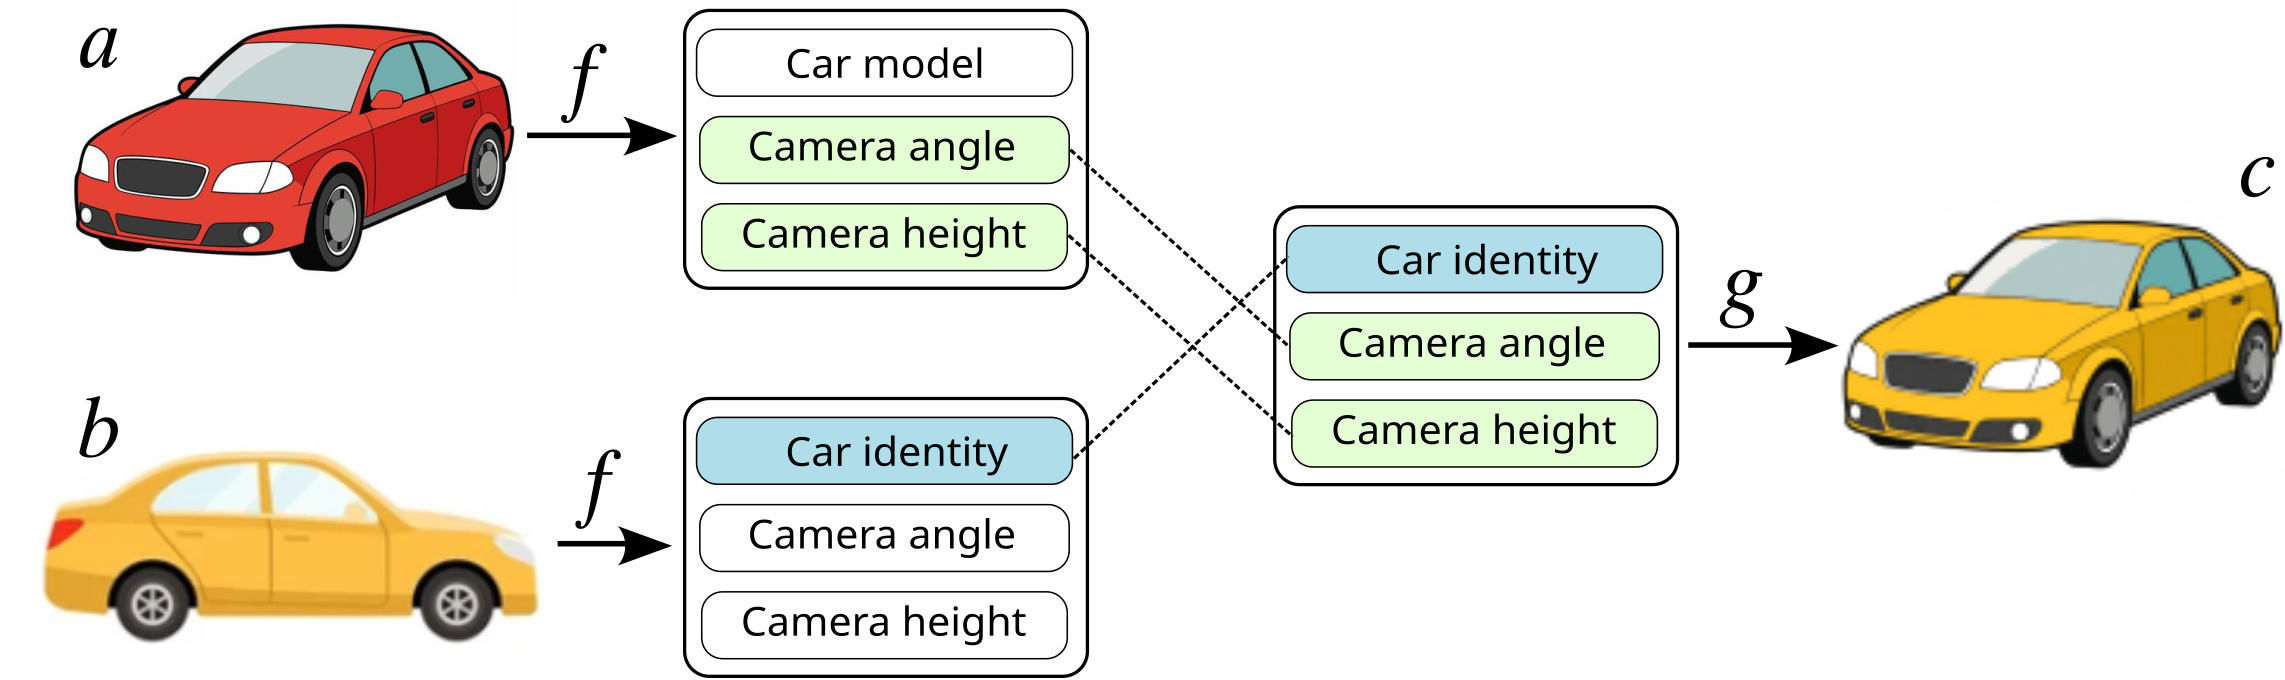
\includegraphics[width=0.9\textwidth]{images/disentangled-representation-learning.png}
    \end{figure}
\end{frame}

\begin{frame}{¿Por qué se eligió el modelo DMRL?}
    \begin{itemize}
        \item \textbf{\textit{Disentangled representation learning}}: 
        \begin{itemize}
            \item Captura preferencias de usuarios sobre factores específicos (e.g., calidad, apariencia) para diferentes modalidades.
            \item Reduce redundancias en la representación de características y mejora la personalización y la explicabilidad.
        \end{itemize}
        \item \textbf{Multimodalidad real}: Información visual y textual simultáneamente.
        \item \textbf{\textit{Attention is all you need}}: Mecanismo de atención para ponderar la los factores según el historial de valoraciones.
    \end{itemize}
\end{frame}

\begin{frame}{Arquitectura de DMRL}
    \begin{figure}
        \centering
        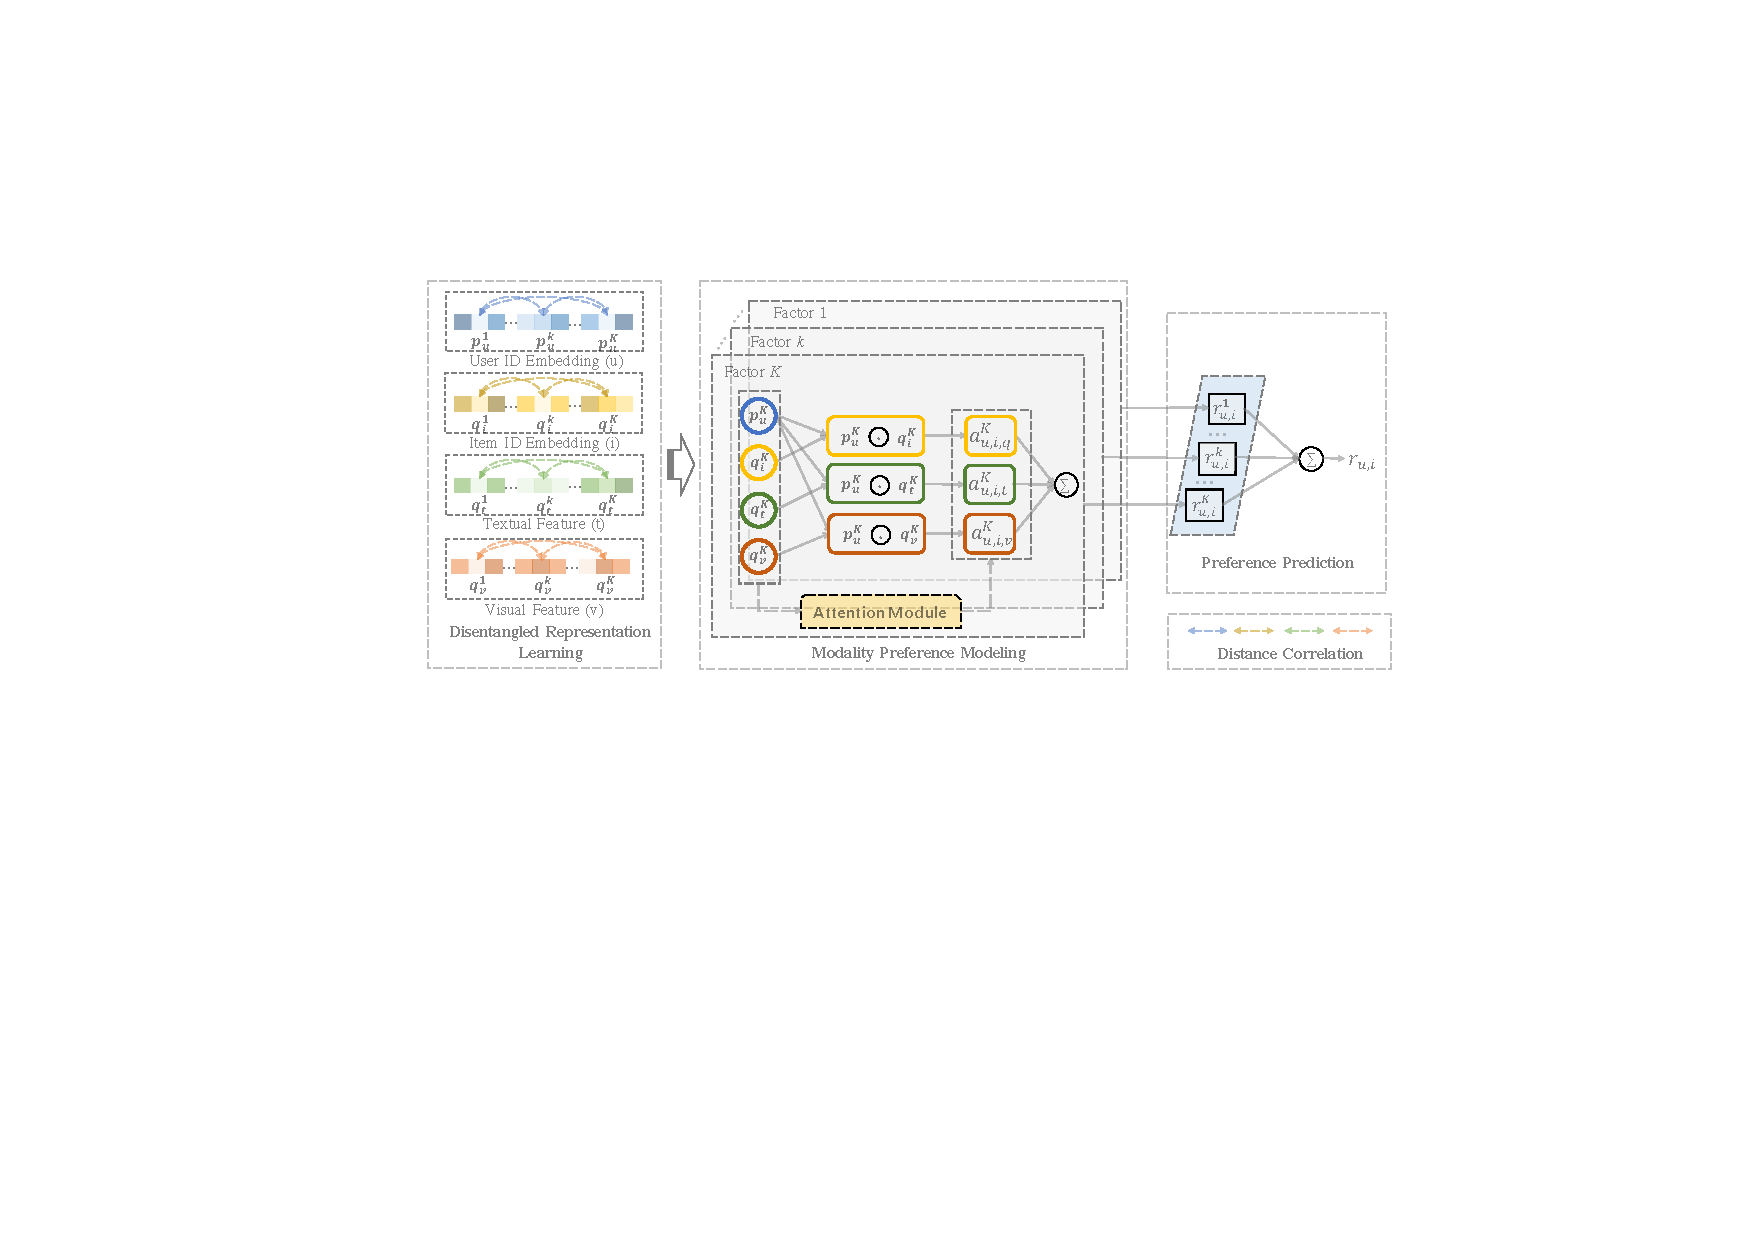
\includegraphics[width=0.9\textwidth]{images/dmrl_arch.pdf}
    \end{figure}
\end{frame}

% Resultados Experimentales Section
\section{Resultados experimentales}

\section*{Extracción de características}

\begin{frame}{Subtítulos: SentenceTransformers}
    \begin{table}[t]{}
        \centering
        \resizebox{\textwidth}{!}{%
            \begin{tabular}{lrll}
                \hline
                \textbf{Rank} & \textbf{Score} & \textbf{Title} & \textbf{Genres} \\ \hline
                1 & 0.6089 & The Battle of Shaker Heights (2003) & Comedy Drama Romance\\
                2 & 0.5546 & Daddy and Them (2001) & Comedy Drama\\
                3 & 0.5522 & The Ugly (1997) & Horror Thriller\\
                4 & 0.5402 & Ajami (2009) & Crime Drama\\
                5 & 0.5324 & A Goofy Movie (1995) & Animation Children Comedy\\ \hline
            \end{tabular}
        }
    \end{table}
\end{frame}

\begin{frame}{Subtítulos: BERT chunks con mean pooling}
    \begin{table}[t]{}
    \centering
    \resizebox{\textwidth}{!}{%
        \begin{tabular}{lrll}
            \hline
            \textbf{Rank} & \textbf{Score} & \textbf{Title} & \textbf{Genres} \\ \hline
            1 & 0.9940 & Toy Story 2 (1999) & Adventure Animation Children Comedy\\
            2 & 0.9903 & Doogal (2006) & Animation Children\\
            3 & 0.9902 & Escape from Planet Earth (2013) & Adventure Animation Comedy Sci-Fi\\
            4 & 0.9899 & Toy Story 3 (2010) & Adventure Animation Children Comedy\\
            5 & 0.9895 & Chicken Little (2005) & Action Adventure Animation Children\\ \hline
        \end{tabular}
    }
\end{table}
\end{frame}

\begin{frame}{Pósters: CNN VGG16 sin PCA}
    \textbf{Extracción:} 25088-D, sólo capas CNN

    \begin{figure}
        \centering
        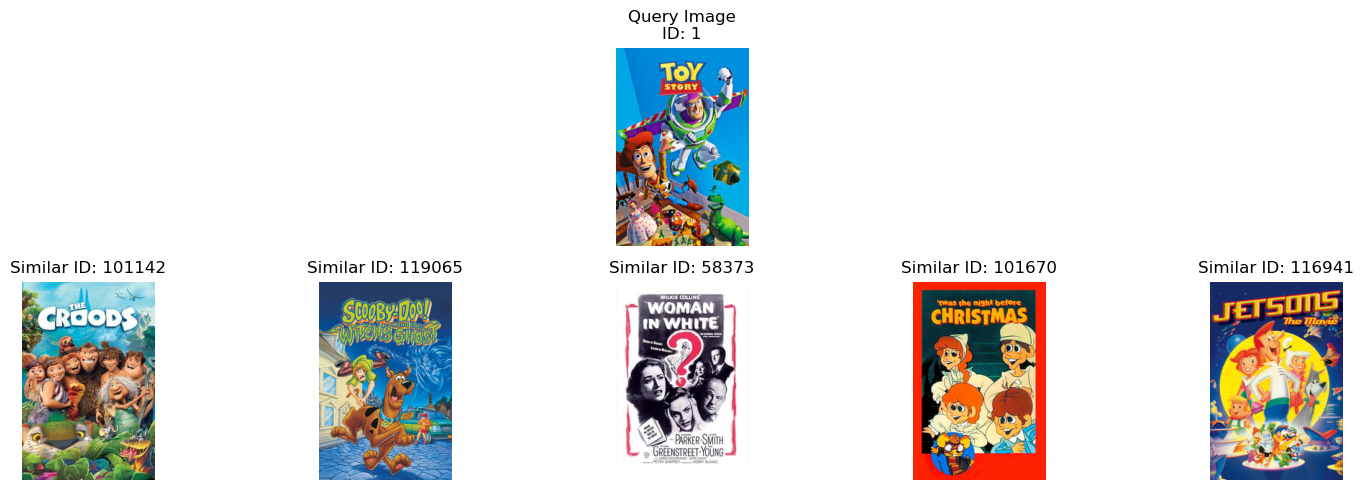
\includegraphics[width=0.9\textwidth]{images/vgg16_cnn_nopca.png}        
    \end{figure}
\end{frame}

\begin{frame}{Pósters: VGG16 con PCA}
   \textbf{Extracción:} 25088-D reducido a 300-D con PCA, sólo capas CNN

    \begin{figure}
        \centering
        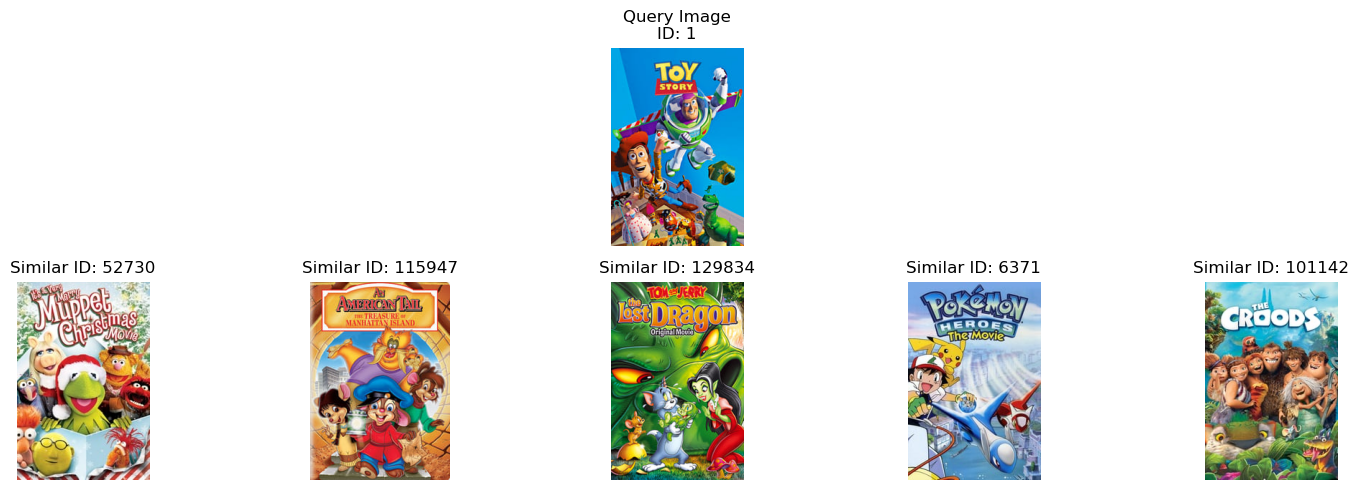
\includegraphics[width=0.9\textwidth]{images/vgg16_cnn.png}
    \end{figure}
\end{frame}

\begin{frame}{Pósters: CNN VGG16 FC2}
    \textbf{Extracción:} 4096-D, tras la segunda capa FC

    \begin{figure}
        \centering
        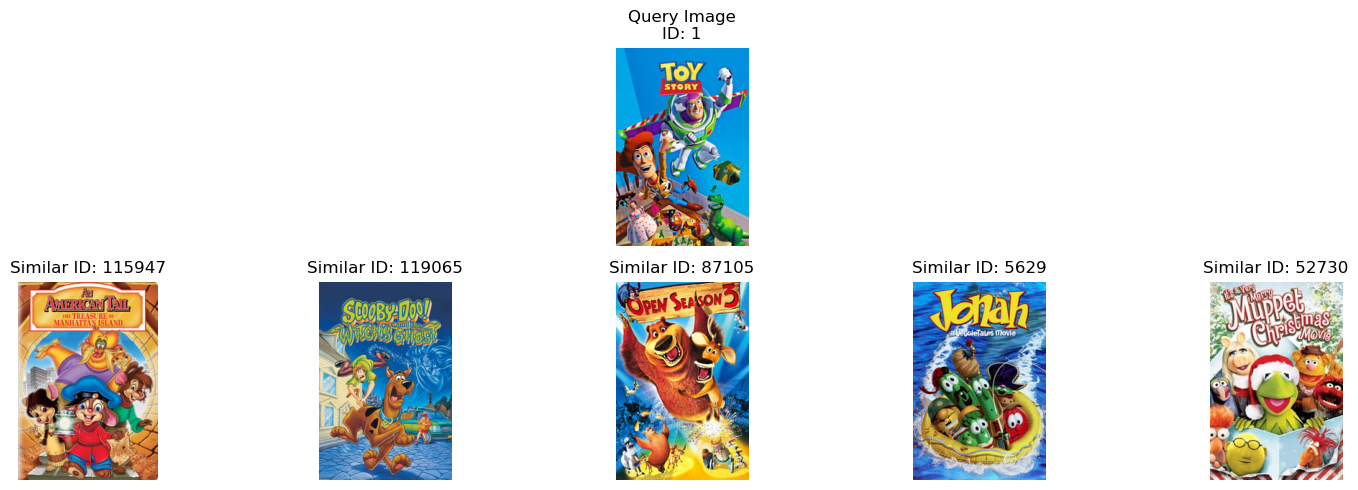
\includegraphics[width=0.9\textwidth]{images/vgg16_fc2_nopca.png}
    \end{figure}
\end{frame}

\begin{frame}{Pósters: Vision Transformers (ViT)}
    \textbf{Extracción:} 1024-D, tras el último transformer del encoder

    \begin{figure}
        \centering
        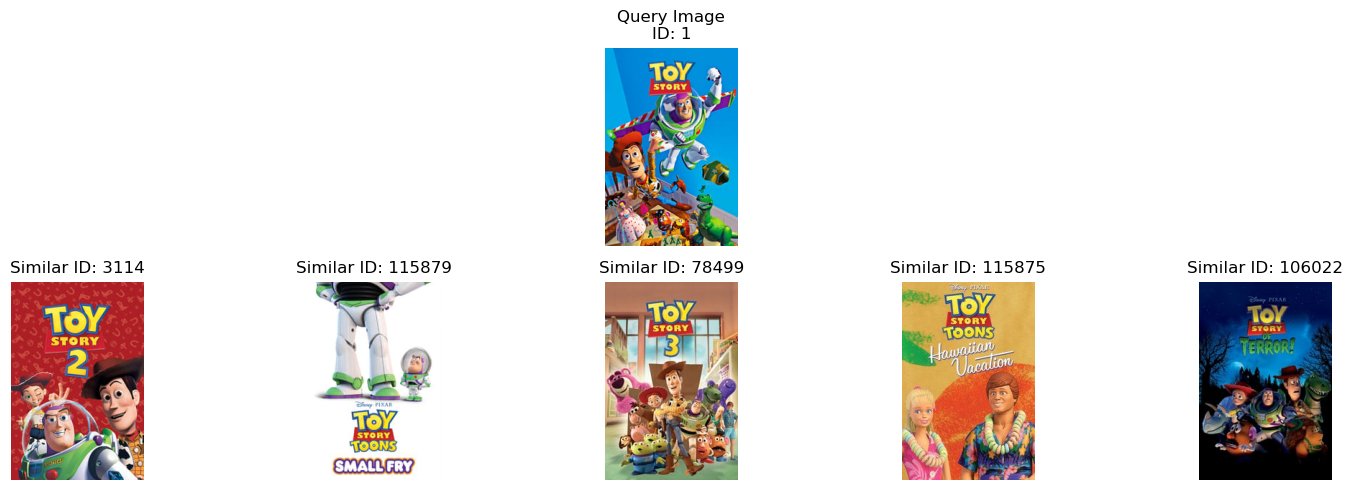
\includegraphics[width=0.9\textwidth]{images/vit_h14.png}
    \end{figure}
\end{frame}

\section*{Resultados del modelo DMRL}

\begin{frame}{Comparación de NDCG y Recall por modelo}
    \begin{figure}
        \centering
        \begin{minipage}{0.48\textwidth}
            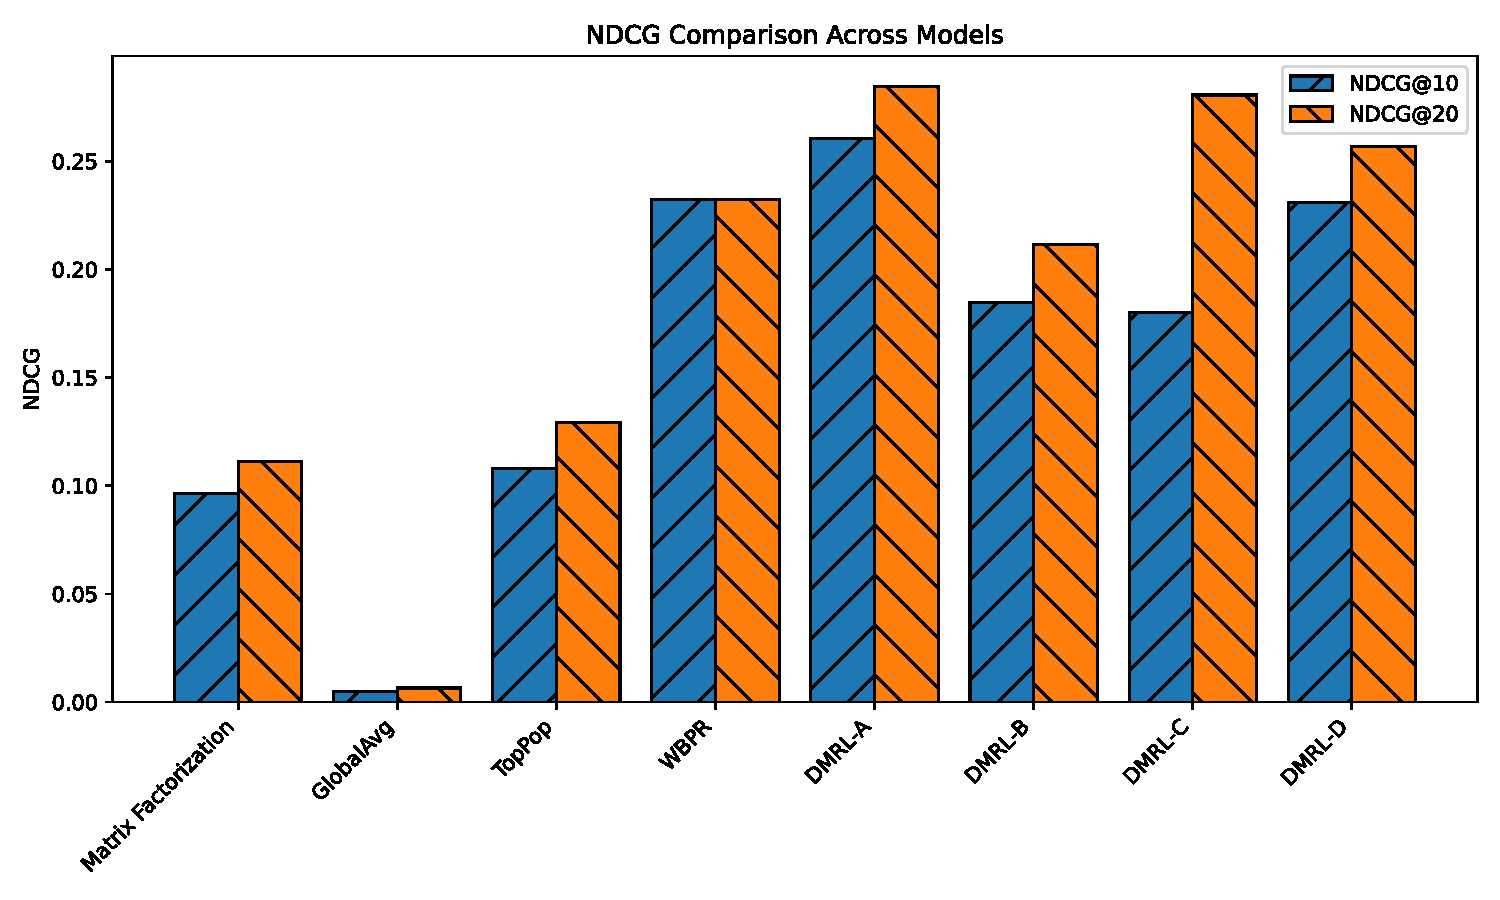
\includegraphics[width=\textwidth]{images/ndcg_comparison.pdf}
            \caption*{NDCG @10,@20}
        \end{minipage}
        \hfill
        \begin{minipage}{0.48\textwidth}
            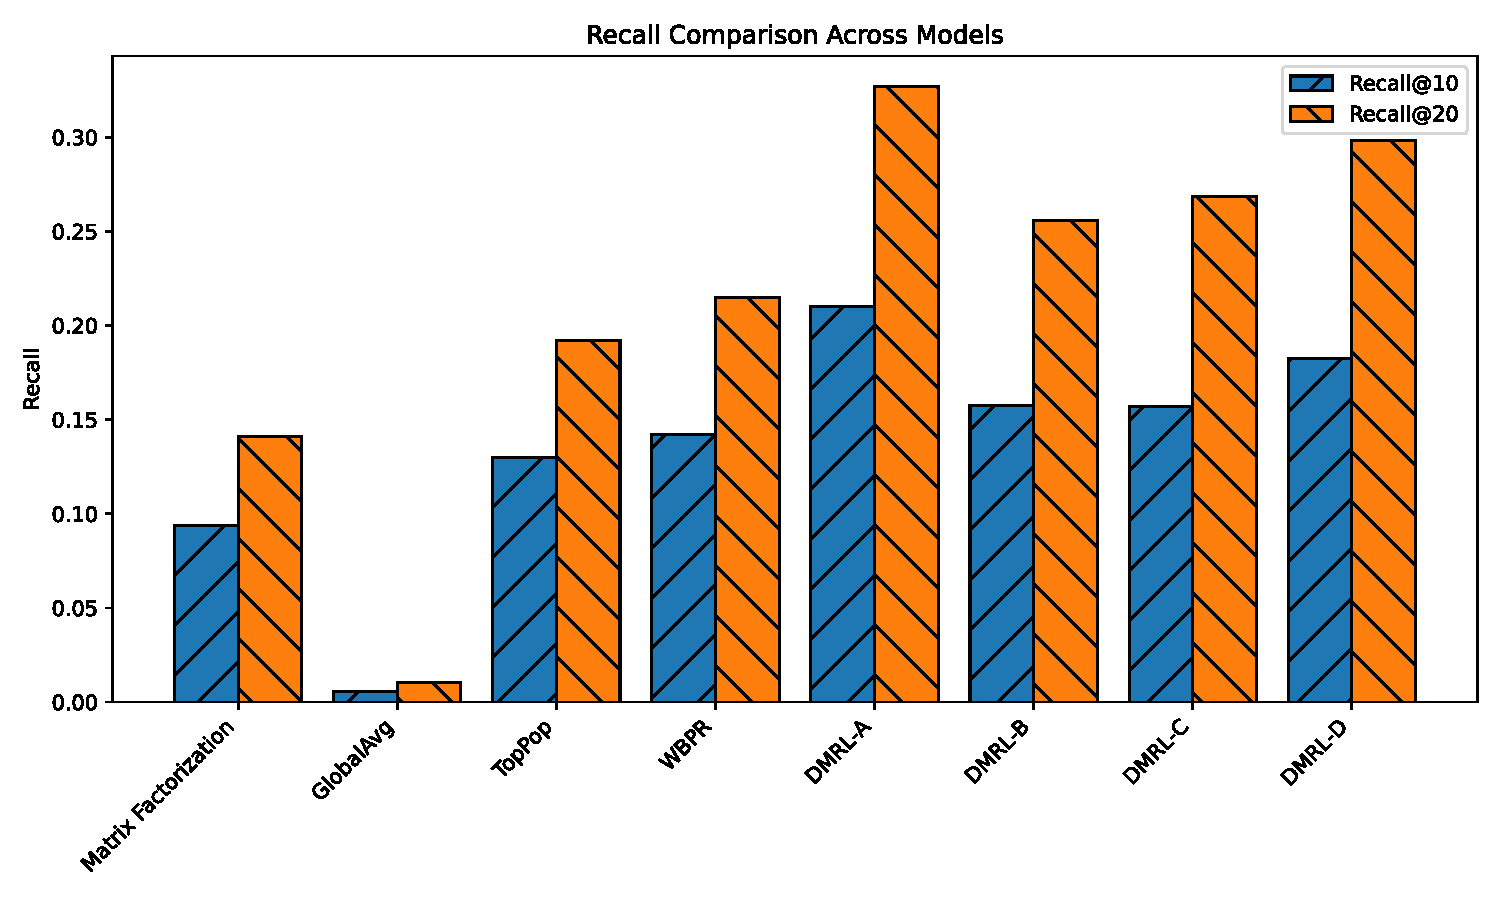
\includegraphics[width=\textwidth]{images/recall_comparison.pdf}
            \caption*{Recall @10,@20}
        \end{minipage}
    \end{figure}
\end{frame}

\begin{frame}{Comparación general de NDCG y Recall}
    \begin{figure}
        \centering
        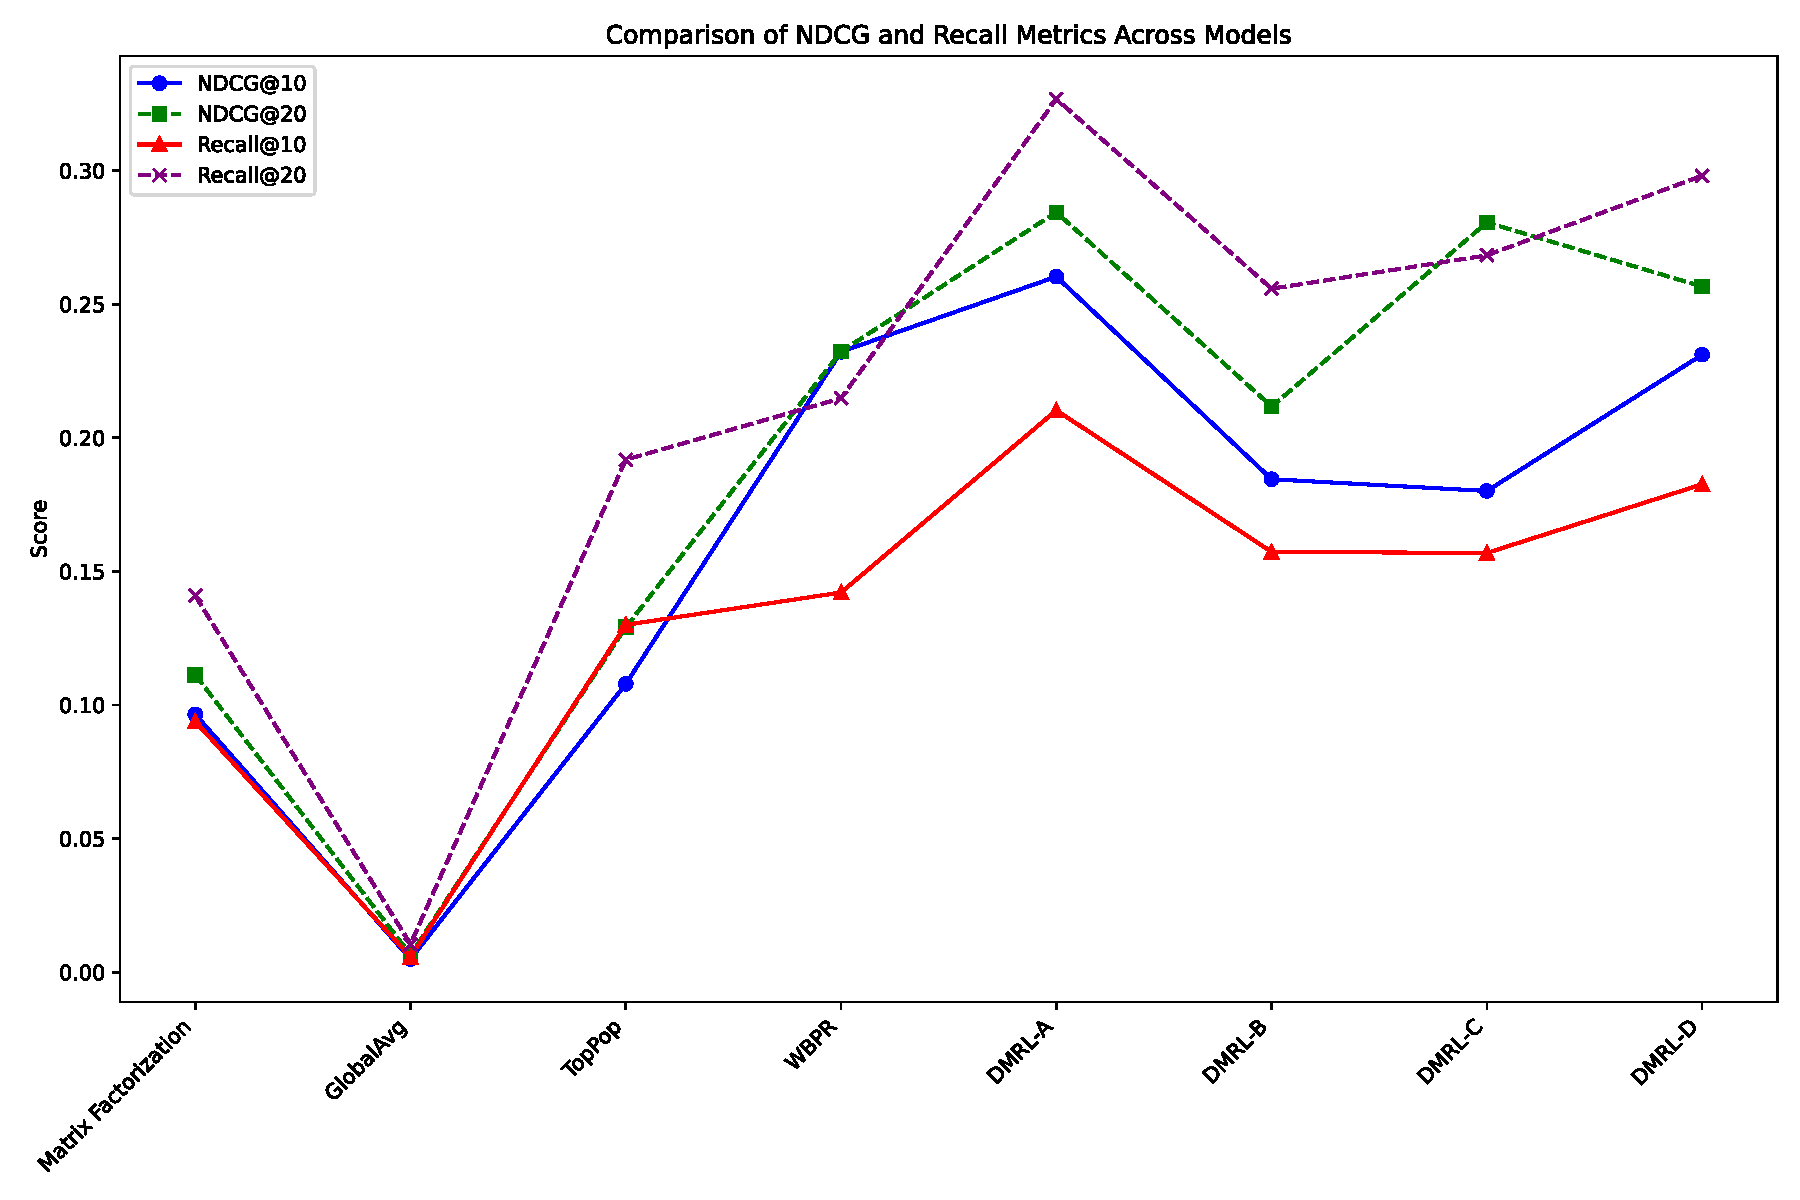
\includegraphics[width=\textwidth]{images/comparison.pdf}
    \end{figure}
\end{frame}

% Architectural Considerations
\section{Consideraciones arquitectónicas}
\begin{frame}{Consideraciones arquitectónicas}
    \begin{itemize}
        \item \textbf{Escalabilidad:} 
        Adaptación para millones de usuarios y catálogos dinámicos con miles de títulos.
        \item \textbf{Recomendaciones en tiempo real:}
        Respuestas en el orden de milisegundos, utilizando embeddings precalculados y técnicas como ANN (\textit{Approximate Nearest Neighbors}).
        \item \textbf{Recomendaciones por lotes:} 
        Uso de pipelines nocturnos para actualizar embeddings, con recomendaciones almacenados en memoria mediante soluciones como Redis.
        \item \textbf{Cambio de modelos:} 
        Enfoque de repositorios centralizados que permite cambios rápidos en los modelos y rollback inmediato en caso de fallos.
    \end{itemize}
\end{frame}

\begin{frame}{Propuesta arquitectónica}
    \begin{figure}
    \centering
        \includegraphics[width=0.9\textwidth]{images/tfm-arch.drawio.pdf}
    \end{figure}
\end{frame}

\section{Ventajas competitivas}
\begin{frame}{Ventajas competitivas}
    \textbf{Características innovadoras:}
    \begin{itemize}
        \item Mejor experiencia de usuario por la sensación de serendipia y novedad de la mayor personalización de recomendaciones.
        \item Mejores recomendaciones a nuevos usuarios y de contenidos relacionados.
        \item Recomendaciones de calidad incluso en la \textit{long tail}.
        \item \textit{Framework} para rápida experimentación y despliegue.
    \end{itemize}
    \textbf{Ventajas clave:}
    \begin{itemize}
        \item Menor \textit{churn rate} por mayor lealtad de usuarios.
        \item Aumento de ingresos por mayores conversión y \textit{engagement}.
        \item Reducción de costes por mejor explotación del catálogo.
        \item Preparada para la rápida evolución de los modelos de IA.
    \end{itemize}
\end{frame}

% Future Work
\section{Trabajo futuro}
\begin{frame}{Trabajo futuro}
    \textbf{Posibles direcciones:}
    \begin{itemize}
        \item Extender el sistema a datasets más grandes como MovieLens-20M.
        \item Integrar modalidades adicionales como grafos de metadatos y sentimiento de reseñas.
        \item Explotar los factores empleados por DMRL tanto para explicabilidad como para herramientas de búsqueda innovadoras.
        \item Validar en entornos reales mediante pruebas A/B.
    \end{itemize}
\end{frame}

% Conclusions
\section{Conclusiones}
\begin{frame}{Conclusiones}
    \begin{itemize}
        \item Los datos multimodales mejoran la personalización de las recomendaciones incluso sin ajuste de hiperparámetros.
        \item Las técnicas de extraccion de las características multimodales son clave en el rendimiento.
        \item DMRL aborda con éxito problemas clave como \textit{cold start} y \textit{long tail}.
    \end{itemize}
\end{frame}

% Closing Slide
\begin{frame}{¡Gracias!}
    \begin{center}
        ¿Preguntas?
    \end{center}
\end{frame}


\end{document}